Käytännössä kaksi ryhmää teknologioille: käyttäjädatan tallennus ja tunnistautumisprotokollat.

Käyttäjädatan tallennus
- passwd (ts tiedosto levyllä tms)
- tietokanta
- AD-kannat (LDAP)

---> käyttäjän datan abstraktoinnin tarve, ehkä mainita, että käyttäjädatan backendejä voi käytännössä olla monta erilaista. Esim. LDAP:n rinnalla tietokannat.

Enivei, luvun pääpaino on protokollissa. Esitellään historia kerberos -> saml -> oauth ja päädytään oauthiin, tarkemmin versioon 2.

Miten käyttäjädataa onko käsitelty ja käsitellään. Kehitys paikallisesti käytetyistä tiedostopohjaisista systeemeistä kohti tietokantoja ja asiaan räätälöihin palveluihin (LDAP). LDAP oleelisin, mutta tutkimuksen kannalta abstraktointi on tärkeä juttu.

Johdanto puoli sivua, alaluvut 0.5-1 sivu.
\subsection{Käyttäjädata}
Miten käyttäjädataa onko käsitelty ja käsitellään. Kehitys paikallisesti käytetyistä tiedostopohjaisista systeemeistä kohti tietokantoja ja asiaan räätälöihin palveluihin (LDAP). LDAP oleelisin, mutta tutkimuksen kannalta abstraktointi on tärkeä juttu.

Johdanto puoli sivua, alaluvut 0.5-1 sivu.
\subsubsection{passwd}
Vanha kunnon /etc/passwd, tästä tunnistautuminen on varmaan lähtenyt käyntiin. Ikävää, kun webiin tunnistautuessa täytyy olla tunnus kyseisellä koneella ja muutenkin ei ole hyvä kun tunnukset siirtyy verkkoa pitkin.
\subsubsection{Relaatiotietokannat}
Käyttäjätietokannat, relaatiokannat lähinnä, ehkä NoSQL.
\subsubsection{LDAP}
Lightweight Directory Access Protocol (LDAP) on X.500 OSI-standardiin perustuva hakemistopalvelu, jota käytetään yleisesti käyttäjätiedon tallennukseen [TODO: lähde]. 1990-luvulla TCP/IP-mallin syrjäytettyä OSI-mallin, myös DAP kävi vanhanaikaiseksi \cite{howes}. Korvaajaksi on noussut LDAP, josta käytetään myös nimeä X.500 Lite \cite{howes}.

LDAP:ssa asiakassovellukset (directory user agent, DUA) keskustelevat puumalliin perustuvan hakemistopalvelimen (directory system agent, DSA) kanssa käyttäen määriteltyä protokollaa (directory access protocol, DAP) \cite{howes}. Asiakassovellukset voivat hakea hakemistopalvelimesta tietoa suodattimiin (filter) perustuvalla lukuoperaatiolla. Suodattimessa voidaan määritellä raja-arvot attribuutin arvolle tai hakea avainsanoilla attribuuteista.

LDAP-tietuille voidaan määritellä pakollisten attribuuttien (esim. etu- ja sukunimi) lisäksi valinnaisia attribuutteja. Tietueet on järjestetty puuhun niiden yksilöivän nimen (distinguished name, DN) mukaan ja ne voi olla hajautettu usealle palvelimelle. Suhteellinen nimi (relative distinguished name, RDN) identifioi tietueen omalla hierarkiatasollaan.

LDAP-tietueella voi olla tunnus sekä salasana ja LDAP-palvelinta voidaan käyttää käyttäjän tunnistautumiseen [TODO: lähde, ehkä rfc4513].

TODO: lisää tekstiä

\subsubsection{Käyttäjädatan abstraktointi}
Tutkimuksen kannalta abstraktointi on oleellista, oikeastaan sillä ei ole ison kuvan kannalta merkitystä, että onko siellä taustalla tietokanta, tiedosto, ldap vai mikä.
\subsection{Rajapintaprotokollat}
Miten käyttäjädataa onko käsitelty ja käsitellään. Kehitys paikallisesti käytetyistä tiedostopohjaisista systeemeistä kohti tietokantoja ja asiaan räätälöihin palveluihin (LDAP). LDAP oleelisin, mutta tutkimuksen kannalta abstraktointi on tärkeä juttu.

Johdanto puoli sivua, alaluvut 0.5-1 sivu.
\subsubsection{Kerberos}
Lähteet:
Enhancing Distributed Web Security Based on Kerberos Authentication Service (\cite{enchancing_distributed_web_security})
Secure Secret-Key Management of Kerberos Service (\cite{secure_secret_key})

Kerberos-protokolla on alunperin MIT:ssa kehitetty tunnistautumisprotokolla, jonka nykyisin käytössä oleva versio 5 julkaistiin alunperin syyskuussa 1993 ja päivitettynä heinäkuussa 2005 [RFC4120]. Se on yleisesti käytössä erilaisissa UNIX-pohjaisissa käyttöjärjestelmissä ja myös Microsoft on käyttänyt sitä oletus-tunnistautumismekanismina Windows 2000:sta lähtien [RFC3244].

Protokollan osapuolia ovat käyttäjä, luotettava kolmas osapuoli ja palvelu, joka vaatii tunnistautumisen. Luotettava kolmas osapuoli on tyypillisesti avaintenjakopalvelin (KDC, Key Distribution Center), joka tunnistaa käyttäjän ja myöntää lipun tunnistautuneelle käyttäjälle. Myönnettyyn lippuun on merkattu palvelu, johon sitä voidaan käyttää ja aikaleima, jonka ajan se on voimassa. Käyttäjä antaa lipun tunnistautumista vaativalle palvelimelle, joka tarkistaa omalla avaimellaan käyttäjän tunnisteen ja aikaleiman, joiden perusteella se myöntää pääsyn palveluun.

Keskitetty tunnistautuminen hajautettuihin järjestelmiin voidaan toteuttaa Kerberos-protokollalla \cite{enchancing_distributed_web_security}. Kerberos on luonteeltaan sopiva hajautettuihin järjestelmiin, koska avaintenjakopalvelin voi jakaa lippuja kaikkiin järjestelmiin, joiden kanssa se on vaihtanut salausavaimet. Tunnistautumispalvelin on tilaton, jolloin sen suorituskykyä voidaan parantaa tarvittaessa skaalaamalla, joten tunnistautumispalvelin voi palvella suurta määrää käyttäjiä \cite{enchancing_distributed_web_security}.

Tunnistautumisessa käytetyt yksityiset avaimet tallennetaan tietokantaan, jolloin on riskinä, että kolmas osapuoli saattaa päästä käsiksi näihin avaimiin ja pystyä allekirjoittamaan lippuja. Jakamalla salaiset avaimet osiin ja hajauttaa se avaintenjakopalvelimeen, tunnistautumista vaativalle palvelimelle ja näiden välillä käytetylle reitittimelle \cite{secure_secret_key}, voidaan parantaa protokollan luotettavuutta. Tämä tekee siitä mahdollisen vaihtoehdon käytetyksi menetelmäksi keskitettyyn tunnistautumiseen hajautetuissa järjestelmistä.

\subsubsection{SAML}
Security Assertion Markup Language (SAML) on OASIS-komitean kehittämä XML-pohjainen avoin standardi tunnistautumiseen ja pääsynhallintaan \cite{saml_spec}. Standardin versio 1.0 julkaistiin marraskuussa 2002, versio 2.0 maaliskuussa 2005 ja viimeksi päivitetty versio lokakuussa 2009.

SAML määrittelee XML-pohjaiset työkalut tunnistautumisen ja pääsynhallinnan toteuttamiseen. Varsinainen toteutus, esimerkiksi mitä tietoja siirretään ja millä tavalla, jätetään SAML:ssä toteuttajan päätettäväksi \cite{dynamic_saml}. Varsinaiset SAML-viestit voivat kulkea esimerkiksi synkronisesti SOAP- ja HTTP-protokollalla. SAML soveltuu avoimena ja XML-pohjaisena protokollana käytettäväksi Web Services -standardilla toteutetuissa web-sovelluksissa.

Noin sivu lisää, jotta selviää mikä SAML loppujen lopuksi on.
\subsubsection{OAuth}
OAuthin kehitystyö alkoi marraskuussa 2006, kun Twitter-pal\-ve\-luun toteutettiin \mbox{OpenID-tukea}. Pian huomattiin, ettei OpenID sovellu käytettäväksi palvelun API-ra\-ja\-pin\-to\-jen kanssa, vaan tarvittiin erillinen pääsynvalvontaprotokolla \cite{oauth_primer}. Siihen asti Twitter-integraatio oli toteutettu pyytämällä käyttäjää antamaan Twitter-tun\-nuk\-sen\-sa ja -salasanansa, joiden avulla palvelu integroitui käyttäjän Twitter-tiliin. Twitterin kehittämä xAuth ja siitä kehittynyt OAuth-protokolla mahdollistavat resurssien käytön ilman käyttäjätunnuksen ja salasanan luovuttamista kolmannelle osapuolelle \cite{oauth2_0}.

OAuthin ensimmäinen versio (1.0) julkaistiin lokakuussa 2007 ja päivitetty versio (1.0a) kesäkuussa 2009 \cite{oauth2_0}. OAuthin versio 2.0 on myös kehitteillä ja se on tarkoitus julkaista marraskuussa 2012 \cite{oauth2_0}. OAuth on määritelty RFC-dokumentissa numero 5849. OAuthin 2.0-version kehitys on ollut vaikeuksissa lähinnä sen jatkuvasti kasvaneiden ominaisuusvaatimusten takia. OAuth 2.0 on kuitenkin käytössä useissa palveluissa, kuten Facebookissa ja GitHubissa, koska OAuth 1.0a:n ominaisuudet eivät ole riittäneet niille. 2.0 helpottaa mm. API-kutsujen tekemistä, koska valtuutusavainten allekirjoitusta on yksinkertaistettu \cite{oauth2_0}.

OAuth on avoin pääsynvalvontaprotokolla hajautetuille web-sovelluksille. Se mahdollistaa käyttäjien resurssien jakamisen palveluiden välillä ilman käyttäjätunnuksen tai salasanan luovuttamista kolmansille osapuolille. Se perustuu erilaisten valtuutusavainten välittämiseen palveluiden kesken \cite{oauth2_0}. Valtuutusavain on allekirjoitettu identiteetintarjoajalla, johon sekä käyttäjä että palvelun toteuttaja luottaa. Muun muassa Facebook tarjoaa avoimen OAuth-rajapinnan, jota web-sovellusten toteuttajat voivat käyttää pääsynvalvonnassaan.

Kuvassa \ref{oauth} on esitetty, kuinka OAuthia käytetään käyttäjän tunnistamiseen. Tunnistautumispalvelin ja käyttäjähallinta voidaan toteuttaa erillisinä palveluina. Tällöin tunnistautumispalvelun antaa pääsyvaltuuden web-sovellukselle, jonka avulla tiedot haetaan käyttäjähallinnasta (kohdat 10 ja 11). Selkeyden vuoksi tunnistautumispalvelun oletetaan toimivan myös käyttäjätietojen jakelijana.

\begin{figure}[!b]
\centering
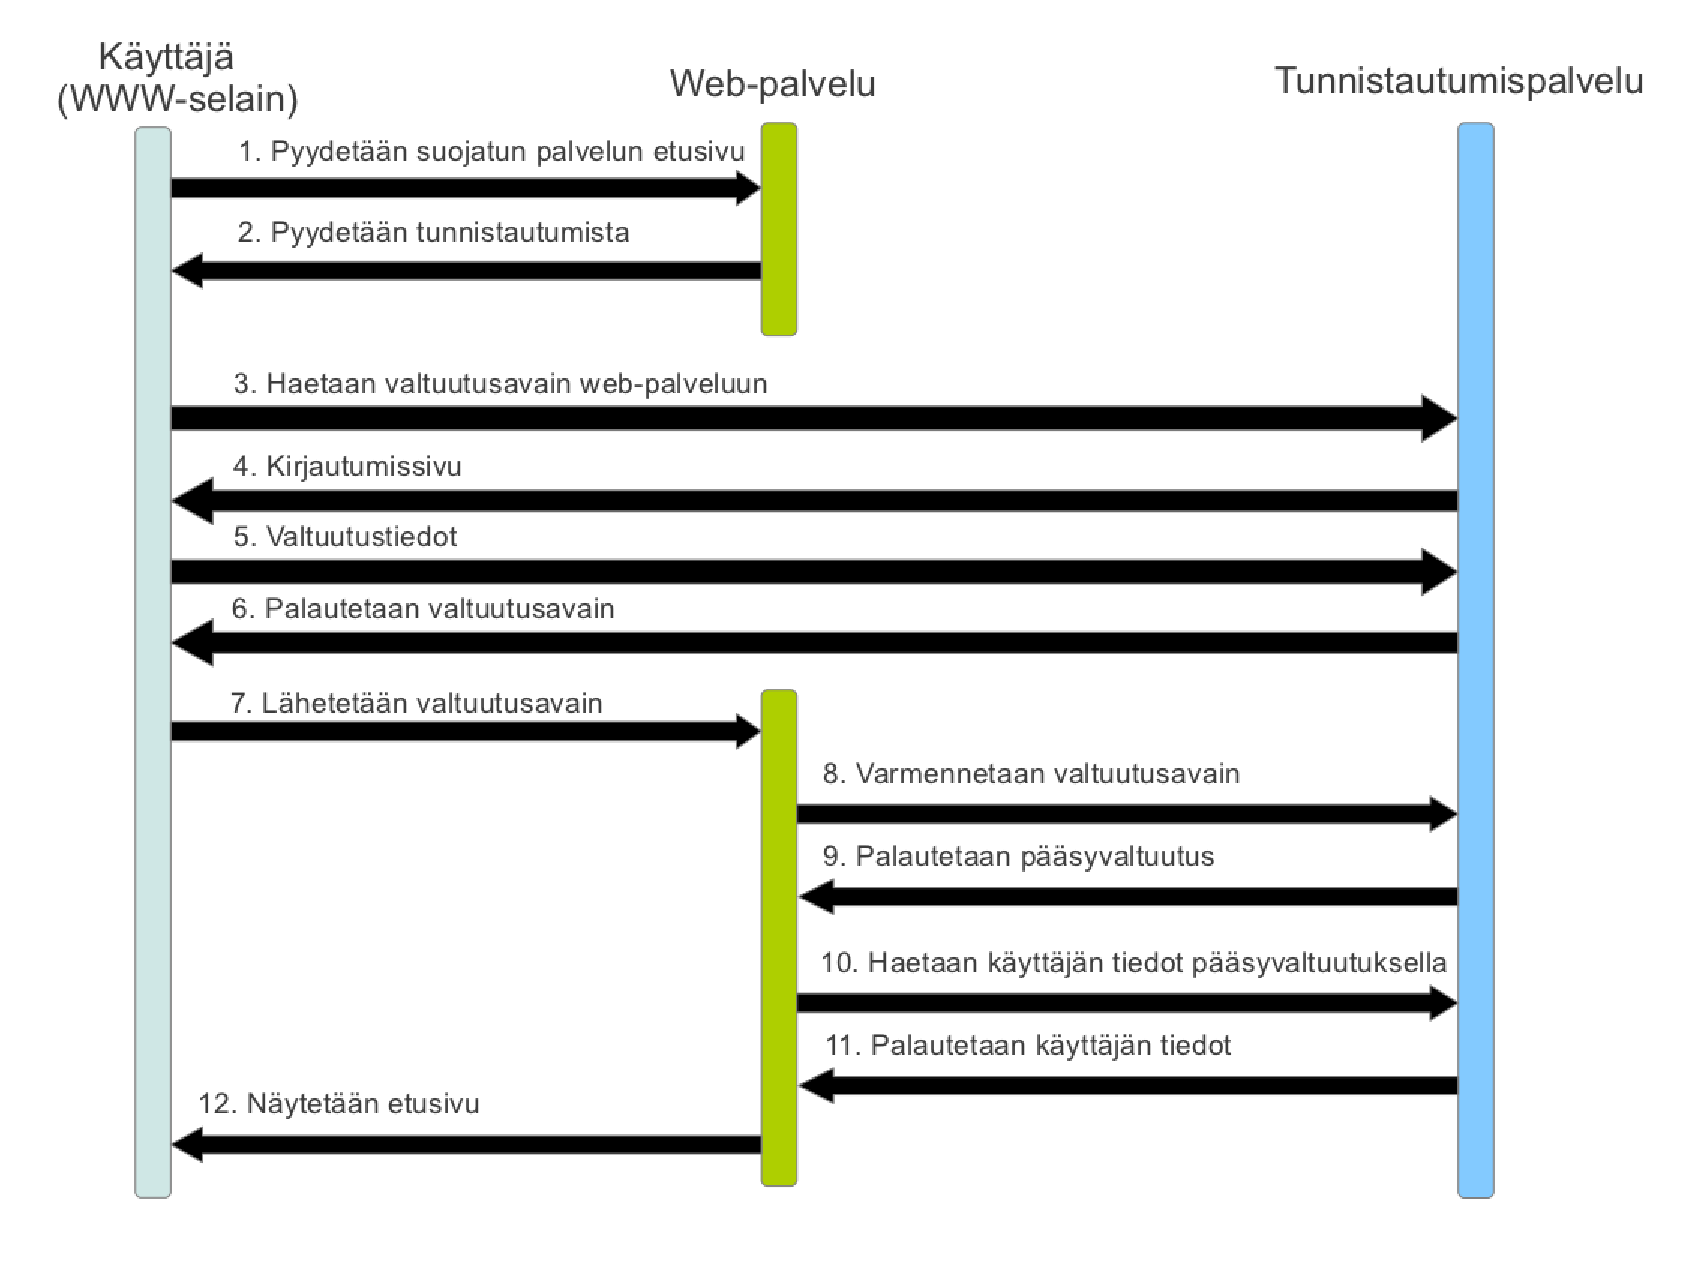
\includegraphics[width=\textwidth]{teknologiat/protokollat/oauth.eps}
\caption{OAuthin toiminta sekvenssikaaviona.}%
\label{oauth}
\end{figure}

OAuthissa valtuutusavaimelle voidaan asettaa erilaisia rajoituksia esimerkiksi sen suhteen, mitä tietoja käyttäjästä annetaan web-sovellukselle tai mihin resursseihin kyseisellä avaimella pääsee käsiksi. Kuvassa \ref{facebook_login} kirjautumisen yhteydessä Porkkanamafialle annetaan oikeus nähdä käyttäjän nimi, profiilikuva, sukupuoli jne. OAuth ei siis ole varsinaisesti tunnistautumisprotokolla, mutta valtuutusavaimen perusteella käyttäjä voidaan yksilöidä: kun käyttäjä kirjautuu myöhemmin uudestaan Porkkanamafiaan, hän hakee valtuutusavaimen Facebookilta, jota käyttämällä Porkkanamafia hakee Facebookista käyttäjän tiedot. Käyttäjän tiedoissa mukana olevalla Facebookin yksilöivällä tunnistenumerolla käyttäjä voidaan todeta samaksi kuin edellisellä kirjautumiskerralla.
\subsection{Vertailu (rajapinnat ja käyttäjädata)}
Keskitetyn tunnistautumispalvelun käyttö on perusteltua, jos ympäristössä on useita käyttäjän tunnistamista vaativia web-sovelluksia. Tunnistautumispalvelun käytöllä ehkäistään käyttäjätietojen kopiointiin liittyviä synkronointiongelmia, kun käyttäjädata on keskitetty yhteen paikkaan. Erityisesti arkaluontoinen data, kuten salasanatiivisteet, kannattaa keskittää, jolloin ne eivät päädy vääriin käsiin yksittäisiin web-sovelluksiin kohdistuneiden tietomurtojen yhteydessä.

Tunnistautumispalvelu mahdollistaa myös muiden kuin järjestelmän ylläpitäjien tuottamien sovellusten käytön organisaation sisäisillä käyttäjätunnuksilla. Käyttämällä luotettavaksi todettuja rajapintoja, voi ylläpito antaa kolmannen osapuolen toteuttamalle web-sovellukselle oikeuden käyttää tunnistautumispalvelua käyttäjän tunnistamiseen. Tällöin käyttäjä ohjataan tunnistautumispalveluun tunnistamisen ajaksi ja web-sovellus saa vain pääsyvaltuuden, jolla sovellus voi hakea käyttäjän tiedot. Käyttäjän tunnistetiedot eivät tule missään vaiheessa tunnistamista tarvitsevan web-sovelluksen tietoon. Näin ollen esimerkiksi Facebook-tunnuksilla voi kirjautua useaan web-sovellukseen, vaikka Facebookilla ei ole tarkkaa tietoa sovelluksien sisäisestä toimintalogiikasta.

Tutkielmassa esitellyn Kapsi ry:n hallintatyökalujen tapauksessa palvelu tullaan toteuttamaan Django-sovelluskehyksellä, mutta myös valmiita toteutuksia on olemassa eri intranet-ympäristöihin. Teknologivalinta tulee tehdä sovellusympäristön mukaan, eikä yksi ratkaisu sovi kaikkiin ympäristöihin. Web-sovelluksen ja tunnistautumispalvelun välinen rajapinta pitää huolen palveluiden yhteensopivuudesta. Rajapinnoiksi on valittavissa useita eri protokollia, kuten Web Services -standardin SAML tai avoimen lähdekoodin yhteisössä syntyneet OpenID ja OAuth. Protokollien käyttö rinnakkain on myös mahdollista, jolloin tunnistautuminen voidaan tehdä esimerkiksi SAML- tai OAuth-protokollalla riippuen web-sovelluksesta.

Tunnistautumiseen liittyvien tehtävien erottaminen yksittäisiltä web-sovelluksilta erillisen palvelun tehtäväksi on palvelusuuntauneiden arkkitehtuurien periaatteiden mukaista. Tällaisten arkkitehtuurien mukaan toteutetuissa sovellusympäristöissä jokaisella web-sovelluksella on oma tarkasti määritelty tehtävä. Kun arkkitehtuurissa on oma palvelu tunnistautumiselle, on pienten yksittäisten komponenttien toteutus helpompaa, koska jokaisen komponentin kohdalla ei tarvitse huolehtia tunnistautumisen toteutuksesta.

Web-sovelluksen ja tunnistamisen erottaminen toisistaan mahdollistaa myös tunnistautumisen tehostamisen ilman muutoksia web-sovellusten toimintaan. Järjestelmässä voidaan ottaa salasanan lisäksi käyttöön toiseen tekijään perustuva tunnistaminen, jolloin esimerkiksi käyttäjän täytyy salasanan lisäksi syöttää matkapuhelimeen lähetetty tunnistekoodi. Web-sovelluksen ja tunnistautumispalvelun välinen rajapinta ei tässä tapauksessa muutu, joten tunnistamisen parantaminen ei edellytä web-sovelluksien muuttamista.

Keskitetyn pääsynvalvonnan toteuttaminen tutkielmassa kuvatuilla periaatteilla on mahdollista. Tällöin tiedot käyttäjien pääsyoikeuksista ympäristön sisällä ovat yhdessä paikassa, joka helpottaa niiden hallinnointia. Esimerkiksi henkilön siirtyessä tehtävästä toiseen, voidaan hänen pääsyvaltuudet muuttaa samasta paikasta. Pääsynvalvontaan voidaan käyttää esimerkiksi tutkielmassa esiteltyjä SAML- tai OAuth-protokollia.

Käyttäjän tunnistamista vaativissa web-sovelluksissa käyttäjän tunnistaminen kannattaa toteuttaa erillisenä komponenttina. Käytettyjen teknologioiden suhteen valinta täytyy tehdä web-sovellusympäristön mukaan, koska kaikkiin ympäristöihin sopivaa ratkaisua ei ole. Tässä tutkielmassa esitellyt periaatteet ovat kuitenkin sovellettavissa eri teknologioita käytettäessä.